\chapter{机械振动}
\section{选择题}
\exercise A

\solve
由图可知,简谐振动的周期介于2至4之间,因此角频率介于0.5$\pi$和$\pi$之间,排除C,D。又由于代入$t=2$,应有$x=A=2$,故仅有A选项满足要求。

\exercise B

\solve
设弹簧振子的振动方程为$x=A\cos(\omega t+\varphi_0)$,则速度方程为$v=\frac{dx}{dt}=A\omega\cos(\omega t+\varphi_0+\frac{\pi}{2})$,故振幅增大一倍,速度亦增大一倍,选B。

\exercise C

\solve
动能与振子速度的平方成正比,且在振子速度最大时,动能等于振动总能量。因此,此时动能与动能总能量的比等于$\cos^2(\omega t+\varphi_0+\frac{\pi}{2})$。又由于此时位移大小为振幅的$\frac{1}{4}$,知$\cos(\omega t+\varphi_0)=\frac{1}{4}$,故$\cos^2(\omega t+\varphi_0+\frac{\pi}{2})=1-\cos^2(\omega t+\varphi_0)=1-\left(\frac{1}{4}\right)^2=\frac{15}{16}$,选C。

\exercise C

\solve
由图可知,$v|_{t=0}=\frac{1}{2}v_{max}$,又由于图像为余弦函数右移后图像,知速度初相位为$-\frac{\pi}{3}$。若设位移初相位为$\varphi_0$,则速度初相位为$\varphi_0+\frac{\pi}{2}=-\frac{\pi}{3}$,因此$\varphi_0=-\frac{5\pi}{6}$,选C。

\exercise A

\solve
机械振动的角速度$\omega=\sqrt{\frac{a_{max}}{x_{max}}}=\sqrt{\frac{a_m}{A}}$,因此周期$T=\frac{2\pi}{\omega}=2\pi\sqrt{A/a_m}$,A选项正确,B选项错误。

通过平衡位置的总能量等于动能$E=\frac{1}{2}mv{_{max}}^2=\frac{1}{2}ma{_m}A$,故CD错误,选A。

\exercise A

\solve
由于起点时刻位移为$\frac{1}{2}A$,A、B选项符合要求。又由于起始时刻向x轴负方向运动,仅有A选项满足要求。

\exercise E

\solve
动能方程只能表示速度的大小,而不能表示初始状态下速度方向,因此最后一定有两个相差$\pi$的可能初始相位,因此选E。

\exercise A

\solve
弹簧振子的劲度系数与长度反比,因此每根短弹簧的劲度系数为3k。并联以后,物体受力为三根弹簧受力之和,因此相当于一根劲度系数为9k的弹簧。因此弹簧振子的周期$T=2\pi\sqrt{\frac{m}{k'}}=\frac{2\pi}{3}\sqrt{\frac{m}{k}}$,选A。

\exercise B

\solve 
由题可知,第二个质点的加速度到达正向最大(对应位移负向最大)时,第一个质点在平衡位置向正向移动。因此第二个点比第一个落后1/4个周期,也即$\pi/2$个相位。因此选B。

\exercise B

\solve
拍频等于两个音叉固有频率的差的绝对值,因此A、B选项满足要求。又由于周期$T=2\pi\sqrt{\frac{k}{m}}$,因此挂上重物后,待测音叉的震动周期变长,频率减小。由于此时的拍频也减小,说明待测音叉的固有频率是高于标准音叉的,选B。

\section{填空题}
\exercise 不是

\solve 
见教材75页,同方向不同频率谐运动的合成后振幅随时间变化,不是简谐运动。

\exercise $0.5\mathrm{cm}$ \quad $x=0.5cos(\pi t+\pi)$

\solve
初始状态速度为0,因此处在位移负向最大状态,故振幅为0.5cm,初相位为$\pi$。又由于频率为0.5Hz,知角频率为$\pi$Hz,即振动方程为$x=0.5cos(\pi t+\pi)$
 
\exercise $\frac{\sqrt{7}}{2}$ \quad $\arctan{\frac{2\sqrt{3}}{3}}$

\solve
\begin{figure}[htbp]
\centering
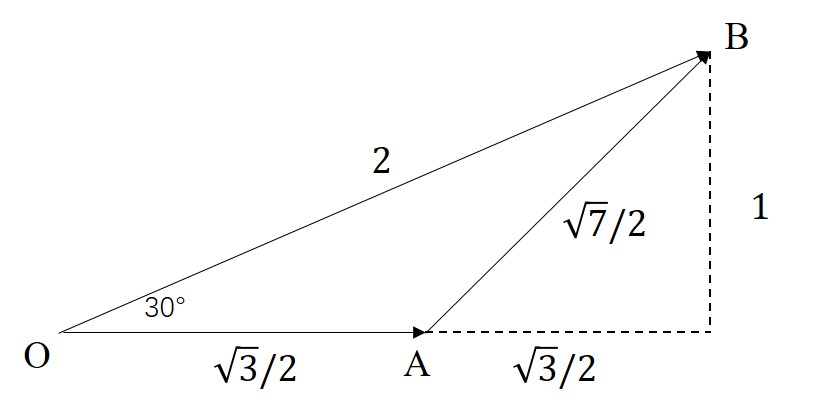
\includegraphics[height=4.7cm,width=9.5cm]{Chp13_13.jpg}
\caption{简谐运动矢量叠加图}
\end{figure}
如图绘制出简谐运动的矢量叠加图,其中OA,AB分别为第一,第二个简谐振动,OB为叠加后的简谐振动。在已知OA、AB大小方向的前提下,由几何关系即可以计算出OB的大小(即第二个简谐振动的振幅)以及两个简谐振动的相位差。

\exercise $\frac{T}{24} \quad \frac{7T}{24}$

\solve
由于速度始终比位移提前1/4个周期,而动能,势能分别与速度的平方、位移的平方成正比,因此当且仅当相位为$\pm\frac{\pi}{4}$或$\pm\frac{3\pi}{4}$ 时,动能与势能相等。因此,在半个周期内,两个动能与势能相等的时刻分别为$t_1=\frac{T}{2\pi}\left(\frac{\pi}{4}-\frac{\pi}{6}\right)=\frac{T}{24}, t_2=\frac{T}{2\pi}\left(\frac{3\pi}{4}-\frac{\pi}{6}\right)=\frac{7T}{24}$。

\exercise $0.03\cos(\frac{\pi}{2}t-\frac{\pi}{2})$

\solve
由图可知,两个简谐运动的振动方程分别为$x_1=0.06\cos(\frac{\pi}{2}t-\frac{\pi}{2})$,$x_2=-0.03\cos(\frac{\pi}{2}t-\frac{\pi}{2})$,相加后即可算出合振动的方程为$x=0.03\cos(\frac{\pi}{2}t-\frac{\pi}{2})$。

\exercise $3$

\solve
由图可知,图像为向右平移了$\frac{\pi}{3}$的余弦曲线,因此初始时刻的相位为$-\frac{\pi}{3}$,另一个x为1的点的相位与初始点关于相位为$\frac{\pi}{2}$对称,因此经过$\frac{2\pi}{3}$的角位移所需的时间为1s,由于一个周期对应$2\pi$的角位移,因此振动的周期为3s。

\exercise $\frac{3}{4}E \quad \frac{1}{4}E \quad \pm\frac{\sqrt{2}}{2}A$

\solve
弹簧振子的弹性势能与位移的平方成正比,因此当位移是振幅的一半时,弹性势能是最大弹性势能的1/4。注意到最大弹性势能与总能量$E$相等,故势能$E_p=\frac{1}{4}E$,动能$E_k=E-E_p=\frac{3}{4}E$。同理,当动能与势能相等,均为总能量一半时,位移的大小应为振幅的$\frac{\sqrt{2}}{2}$倍,即位移为$\pm\frac{\sqrt{2}}{2}A$。

\exercise $0.05\mathrm{m}\quad -\arccos{\frac{3}{5}}$

\solve
对$x$求导有$v=3A\cos(3t+\varphi+\frac{\pi}{2})$,故由题意知,$x(0)=A\cos\varphi=0.03,v(0)=3A\cos(\varphi+\frac{\pi}{2})=0.12$,联立两式即可解出$A$与$\varphi$的值。

\exercise $\sqrt{2}:\sqrt{3}$

\solve
单摆的周期$T=2\pi\sqrt{\frac{l}{g}}$,因此周期正比于绳长的平方根。由于左右两边的绳长比为2:3,周期比为$\sqrt{2}:\sqrt{3}$。

\exercise

\solve
\begin{figure}[htb]
\centering
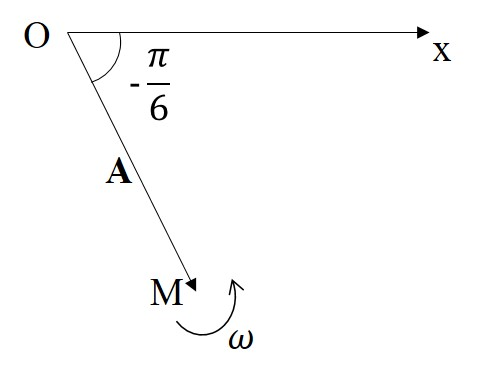
\includegraphics[height=3.7cm,width=5cm]{Chp13_20.jpg}
\caption{旋转矢量图}
\end{figure}
具体绘图方法见教材72页。

\section{计算题}
\exercise

\solve
(1)加速度$a=\frac{F}{m}=-2x$,因此角频率$\omega=\sqrt{\frac{a}{-x}}=\sqrt{2}$,故周期为$T=\frac{2\pi}{\omega}=\sqrt{2}\pi$。

(2)由于动能的最大值等于势能的最大值,有:$E_{\text{动}max}=E_{\text{势}max}=\frac{1}{2}kA^2=0.0675$J

\exercise

\solve
(1)振动的角频率$\omega=\frac{2\pi}{T}=\pi$Hz。撤去外力后,物体处于正向位移最大,负向加速度最大的状态,而撤去外力前,物体平衡。因此,撤去的外力大小等于物体振动过程中的受力最大值,即$F=ma_{max}=mA\omega^2=0.493$N

(2)弹簧的弹性系数$k=F/A=4.93$N/m,因此振动系统的总能量(与弹性势能最大值相等)为$E_{max}=\frac{1}{2}kx^2=0.0247$J。由于势能与相对平衡位置的位移的平方正比,当物体在平衡位置以下5cm,即最大位移的1/2处时,势能是最大势能(也就是总能量)的1/4,因此$E_p=\frac{1}{4}E_{max}=0.00617$J,而动能$E_ k=E_{max}-E_ p=0.0185$J

\exercise

\solve
设单摆振动方程为$x=A\cos(\omega t+\varphi_0)$,则速度方程为$v=\frac{dx}{dt}=A\omega\cos(\omega t+\varphi_0+\frac{\pi}{2})$。故由题意知,
\begin{equation*}
  \left\{
   \begin{array}{c}
   x(0)=A\cos{\varphi_0} = -5  \\
   v(0)=A\omega\cos(\varphi_0+\frac{\pi}{2}) = -10  \\
   \omega=\sqrt{\frac{g}{l}}=2.89{\rm Hz}   \\
   \end{array}
  \right.
\end{equation*}
解方程得,振幅$A=6.08$cm,初相${\varphi_0}=1.57$rad\\
另一方面,周期$T=\frac{2\pi}{\omega}=2.18$s

\exercise

\solve
以向右为正方向,设A的加速度为$a$,相对弹簧自由状态的位置为$x$。首先对A水平受力分析,A受到弹簧的力$F_1=-kx$,以及AB间绳的拉力$F_2$。为求出$F_2$,再对滑轮受力分析。滑轮转动惯量$J=\frac{mR^2}{2}$,角加速度$\beta=a/R$,右端拉力为$m_2g$,因此左端拉力$F_2=m_2g-\frac{J\beta}{R}=m_2(g-a)-0.5ma$
故A的合力$F=F1+F2=-kx+m_2(g-a)-0.5ma$,于是可以推导出a的加速度方程:
\begin{equation*}
\begin{split}
a=\frac{-kx-0.5ma+m_2(g-a)}{m_1}\\
a=\frac{-kx-0.5ma+m_2g}{m_1+m_2}\\
(1+\frac{m}{2m_1+2m_2})a=-\frac{k}{m_1+m_2}x+\frac{m_2}{m_1+m_2}g\\
a=-\frac{2k}{2m_1+2m_2+m}(x+x_0)
\end{split}
\end{equation*}
其中,$x_0=\frac{2m_2g}{2k}$。于是,角频率$\omega=\sqrt{\frac{a}{-x}}=\sqrt{\frac{2k}{2m_1+2m_2+m}}$
